\chapter{Implementation}
\label{sec:implementation}
We created an implementation of our system as a proof of concept. Our system uses a web based GUI for the visualizations while the backend processing is done using Spark\citep{shanahan2015large}. We borrowed from the MapReduce implementation of Salient Features from the Data Polygamy Framework\citep{chirigati2016data}. There are three main stages in our system pipeline: Preprocessing, User Input, and Explanation Visualization. The preprocessing stage is different for each approach to explanation. The user input stage can be divided into two further parts: The user observation, and the type of explanation the user is interested in. An example of the explanation approach would be intervention. The user observation can be one of the attributes the user wants to observe e.g. a mathematical expression spanning several aggregate queries.

\section{Aggravation}
\label{aggravation_impl}
The aggravation approach that we use makes several optimizations to the naive approach one may come up with. A naive approach may consider each candidate explanation and calculate the degree of explanation by aggravation for each one. However, using such an approach would take a long time. If the attribute which we are looking into for explanation has $m$ possible values, it would take $O(m)$ queries to come up with top explanations. If we have $r$ rows in our dataset and each observation query has a linear time complexity, our total time complexity would be $O(rm)$. We can reduce the time complexity by a large factor if we make each candidate explanation cover a larger range of the dataset.

%Talk about bucketing
As mentioned in Section~\ref{sec:aggravation}, we use bucketing to reduce the number of permutations. We use the standard deviation, $\sigma$, of each attribute to separate values which are near the average from the others. We can get the minimum and standard deviation of each attribute over a single iteration of our table in $O(r)$ time. Since the bucket for each value of the attribute can be calculated in constant time, we create a new table containing the bucket value of the attribute in $O(r)$ time.

%Talk about grouping
Since we bucketed our data, the number of candidate explanations have been reduced to $O(\big(\frac{m}{\sigma}\big))$. However, there is still room for improvement. Our observation is always an aggregate query. If we group on the explanation attributes, we can still get all of the corresponding values of the observation in one iteration of the data, making our time complexity $O(r)$.

%Talk about zoning
Another component of our system is spatial data. Our system is designed to handle spatial observations and explanations. When given a spatial observation, our system filters out the data with the spatial predicate given in the observation. The remaining data is used just like any other explanation task. Spatial Explanations, on the other hand, require a bit more work. Given a set of polygons, doing a spatial join with the data is a very expensive process. Our system performs a spatial join once and assigns each tuple an ID based on which polygon it belongs to. The ID can now be used as a regular attribute for the explanation.

\section{Intervention}
\label{intervention_impl}

%Talk about grouping
Intervention is another approach that our system uses. Some of the work we did to optimize aggravation cannot be used to improve the time complexity of intervention. This is because intervention looks at the effect of removing data. While we could use a single iteration of the data for aggravation. We cannot do so for intervention because removing one portion of the data completely changes what the observation looks like. We can still use bucketing to reduce the number of combinations.


\section{Hierarchical Intervention}
\label{sec:hie_impl}
Hierarchical intervention is an improvement on top of the intervention approach. The main idea behind hierarchical intervention is to group spatially colocated points/polygons together in an attempt to improve explanations. We use a partitioning algorithm to create clusters. The base case of our algorithm consists of clusters with a single node each. This makes the results of intervention a subset of the results of hierarchical clustering. Algorithm~\ref{alg:hie} highlights the algorithm that we used for our implementation of greedy hierarchical clustering. Note that each level in the hierarchy is a set cover of all the nodes.


% Talk about clustering
\begin{algorithm}
\caption{Algorithm for Hierarchical clustering}\label{alg:hie}
\begin{algorithmic}[1]
\Procedure{Cluster}{$max\_radius,points$}
      \State $input: max\_radius, points$
      \State $output: hierarchy\_of\_clusters$
       \State $level \gets 0$

      \State $isBaseCase \gets false$
      \While{isBaseCase = false}
          \State $level \gets level + 1$
          \State $levelRadius \gets \frac{max\_radius}{2.0^{level}}$

           \State $hierarchy \gets \emptyset$

          \State $unusedPoints \gets \emptyset$

          \For{$point \gets points$}
              \State $unusedPoints \gets unusedPoint \cup point$
          \EndFor

          \While{$unusedPoints.size > 0$}
              \State $cluster \gets \emptyset$

              \State {$centroid \gets $random point from points}

              \For{$point \gets unusedPoints$}
                  \If{point inside levelRadius}
                      \State $cluster \gets cluster \cup point$
                      \State $unusedPoint \gets unusedPoints - point$
                 \EndIf
              \EndFor

              \State $hierarchy \gets hierarchy \cup cluster$

          \EndWhile
        \algstore{myalg}
    \end{algorithmic}
    \end{algorithm}
    \begin{algorithm}
    \begin{algorithmic} [1]
    \algrestore{myalg}
          \State $hierarchy\_of\_clusters \gets hierarchy\_of\_clusters \cup \{level,hierarchy\}$

          \State $isBaseCase \gets true$

          \For{$cluster \gets heirarchy$}
              \If {$cluster.size > 1$}
                  \State $isBaseCase \gets false$
              \EndIf
          \EndFor
      \EndWhile
      \State \textbf{return} $hierarchy\_of\_clusters$

\EndProcedure
\end{algorithmic}
\end{algorithm}

\begin{figure}
%   \begin{algorithmic}[1]
%   %     \State $input: max_radius, points$
%   %     \State $output: hierarchy_of_clusters$
%   %      \State $level \gets 0$

%   %     \State $isBaseCase \gets false$
%   %     \While{isBaseCase = false}
%   %         \State $level \gets level + 1$
%   %         \State $levelRadius \gets \frac{max_radius}{2.0^{level}}$

%   %          \State $hierarchy \gets \emptyset$

%   %         \State $unusedPoints \gets \emptyset$

%   %         \For{$point \gets points$}
%   %             \State $unusedPoints \gets unusedPoint \cup point$
%   %         \EndFor

%   %         \While{$unusedPoints.size > 0$}
%   %             \State $numShapes \gets unusedPoints.size$
%   %             \State $cluster \gets \emptyset$

%   %             \State $centroid \gets random point from points$

%   %             \For{$point \gets unusedPoints$}
%   %                 \If{$point inside levelRadius$}
%   %                     \State $cluster \gets cluster \cup point$
%   %                     \State $unusedPoint \gets unusedPoints - point$
%   %             \EndFor

%   %             \State $hierarchy \gets hierarchy \cup cluster$

%   %         \EndWhile
%   %         \State $hierarchy_of_clusters \gets hierarchy_of_clusters \cup \{level,hierarchy\}$

%   %         \State $isBaseCase \gets true$

%   %         \For{cluster \gets heirarchy}
%   %             \If {cluster.size > 1}
%   %                 \State $isBaseCase \gets false$
%   %             \EndIf
%   %         \EndFor
%   %     \EndWhile
%   %     \State \textbf{return} $hierarchy_of_clusters$
%   \end{algorithmic}
\end{figure}

% \renewcommand{\lstlistingname}{Algorithm}% Listing -> Algorithm
% \begin{lstlisting}[language=JAVA, caption=Algorithm for Hierarchical clustering, label=alg:hie]
% int level = 0;
% // Base Case. Each cluster contains one shape
% boolean isBaseCase = false;
% while(!isBaseCase){
%     level += 1;
%     // radiusL0 contains all points (Hypotenuse of MBR)
%     Double levelRadius = radiusL0 / Math.pow(2.0, level);

%     // Initialize hierarchy
%     ArrayList<List<Integer>> heirarchy = new ArrayList<>();

%     // Initialize a list containing all the points that are not in any cluster
%     ArrayList<Integer> unusedPoints = new ArrayList<>();
%     for(Integer objectId: shapemap.keySet()){
%         unusedPoints.add(objectId);
%     }

%     // Add points to a cluster while they're unused
%     while(unusedPoints.size()>0){
%         int numShapes = unusedPoints.size();
%         ArrayList<Integer> cluster = new ArrayList<>();
%         // Randomly select a shape
%         int pivot =  (int) Math.floor(Math.random() * numShapes);

%         // Get all shapes in radius
%         Point centroid = shapemap.get(unusedPoints.get(pivot)).getCentroid();

%         Iterator<Integer> unusedIter = unusedPoints.iterator();
%         while(unusedIter.hasNext()){
%             Integer objectId = unusedIter.next();
%             Point shapeCenter = shapemap.get(objectId).getCentroid();
%             if(shapeCenter.distance(centroid)<levelRadius){
%                 cluster.add(objectId);
%                 unusedIter.remove();
%             }
%         }

%         heirarchy.add(cluster);
%     }

%     HeirarchicalCluster.put(level, heirarchy);

%     // Check if we reached the base case level
%     isBaseCase=true;
%     for(List<Integer> cluster: heirarchy){
%         if(cluster.size() > 1){
%             isBaseCase = false;
%             break;
%         }
%     }
% }
% \end{lstlisting}

While greedy hierarchical clustering helps in increasing the domain for the degree of explanation by intervention, the random selection of seed points makes the rate of change of influence and intensity(Section~\ref{sec:extending_hi}) over the levels of hierarchy very volatile. Our point is illustrated by fig.~\ref{fig:hieint_passenger_count}. The red line represents influence while the blue line represents intensity. One would expect the curves to be logarithmic. However, they more closely resemble a sinusoidal function.
\begin{figure}[h]
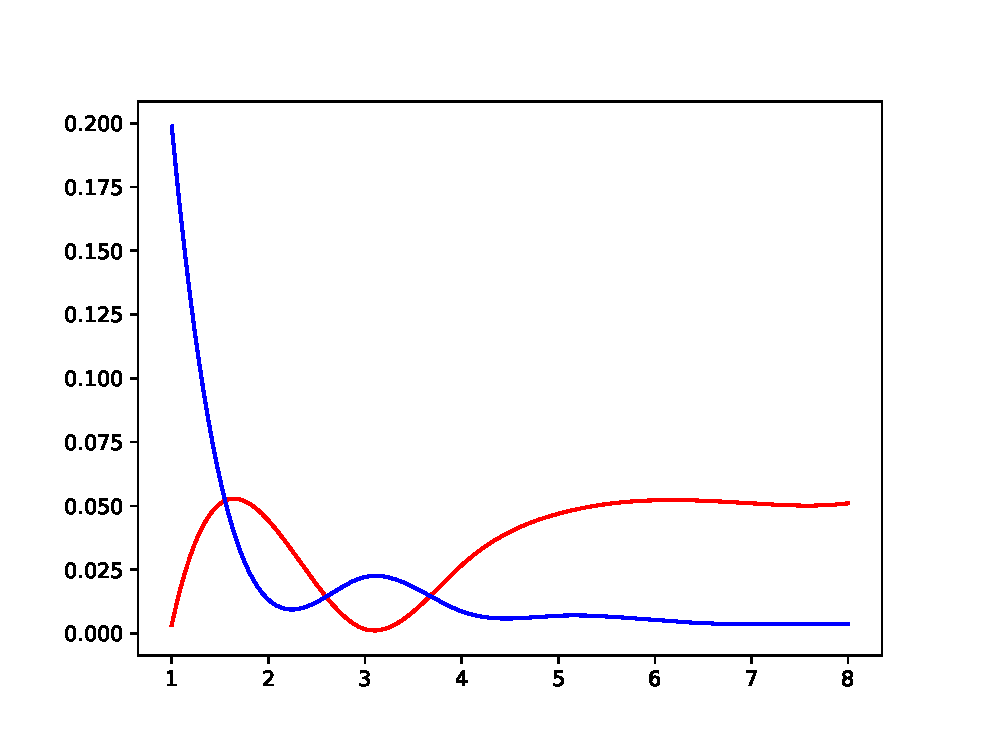
\includegraphics[width=\columnwidth]{hieint_passenger_count}
\caption{Comparison of Influence and Intensity against the level of hierarchy with average passenger count as observation}
\label{fig:hieint_passenger_count}
\end{figure}

In order to try to counter this problem, we used k means clustering. Algorithm~\ref{alg:hie} highlights our implementation of k-means clustering centered around our problem. The algorithm is designed to find the clusters based on a heuristic of giving more preference to balanced clusters i.e. each cluster has a similar number of points.


\begin{lstlisting}[language=JAVA, caption=Algorithm for K means, label=alg:kmeans]
public static HashMap<Point, List<PointDatum>> cluster(PointDatum[] pointData, int k, int numRuns){
    // Generate Cluster Combinations
    ArrayList<Point[]> clusterPossibilities = new ArrayList<>();
    for(int i = 0; i<numRuns; i++){
        clusterPossibilities.add(clusterOnce(pointData, k));
    }

    // Select the best combination
    HashMap<Point, List<PointDatum>> bestClustering = null;
    double bestDistance = Double.MAX_VALUE;
    for(Point[] possibility: clusterPossibilities){
        HashMap<Point, List<PointDatum>> tempCluster = getCluster(possibility, pointData);
        double kdistance = getKMeansDistance(tempCluster);
        if(kdistance<bestDistance){
            bestDistance =kdistance;
            bestClustering = tempCluster;
        }
    }

    return bestClustering;
}

private static double getKMeansDistance(HashMap<Point, List<PointDatum>> clusters){
    double max_distance = Double.MIN_VALUE;
    double min_distance = Double.MAX_VALUE;

    Set<Point> centroids = clusters.keySet();

    for(Point centroid: centroids){
        double clusterWeight = getClusterWeight(clusters.get(centroid));
        if(clusterWeight>max_distance){
            max_distance = clusterWeight;
        }
        if(clusterWeight<min_distance){
            min_distance = clusterWeight;
        }
    }

    return Math.abs(max_distance-min_distance);
}


private static double getClusterWeight(List<PointDatum> pointDatum){
    double clusterWeight = pointDatum.stream()
            .map(pd->{return pd.getValue();})
            .reduce((value1,value2)->{return value1+value2;}).get();
    return clusterWeight;
}

private static HashMap<Point, List<PointDatum>> getCluster(Point[] centroids, PointDatum[] pointData){
    // Form clusters by assigning point to nearest centroid
    HashMap<Point, List<PointDatum>> clusters = new HashMap<>();

    for(Point centroid: centroids){
        clusters.put(centroid, new ArrayList<>());
    }

    for(PointDatum pointDatum: pointData){
        Point closestCentroid = null;
        // Find closest centroid
        for(Point centroid: centroids){
            if(closestCentroid==null){
                closestCentroid = centroid;
            }else if(centroid.distance(pointDatum.getPoint()) < closestCentroid.distance(pointDatum.getPoint())){
                closestCentroid = centroid;
            }
        }

        clusters.get(closestCentroid).add(pointDatum);
    }

    return clusters;
}

static Point[] clusterOnce(PointDatum[] pointData, int k){
    // Select centroids at random
    ArrayList<Point> centroids = new ArrayList<>();

    ArrayList<Integer> selectedIndices = new ArrayList<>();
    for(int i=0; i<k; i++){
        Integer randomIndex = (int)Math.floor(Math.random()*pointData.length);
        while(selectedIndices.contains(randomIndex)){
            randomIndex = (int)Math.floor(Math.random()*pointData.length);
        }
        selectedIndices.add(randomIndex);

        centroids.add(pointData[randomIndex].getPoint());
    }

    GeometryFactory gf = new GeometryFactory();

    // While True
    while(true) {
        // Get cluster
        HashMap<Point, List<PointDatum>> clusters = getCluster(centroids.toArray(new Point[centroids.size()]), pointData);

        // Update centroids
        ArrayList<Point> newCentroids = new ArrayList<>();
        for(Point centroid: centroids){
            // Get cluster
            List<PointDatum> cluster = clusters.get(centroid);

            // Find average point based on weightage
            double sum_x = 0;
            double sum_y = 0;
            double num_values = 0;

            for(PointDatum pointDatum:cluster){
                sum_x += pointDatum.getPoint().getX() * pointDatum.getValue();
                sum_y += pointDatum.getPoint().getY() * pointDatum.getValue();
                num_values += pointDatum.getValue();
            }

            Point avg_point = gf.createPoint(new Coordinate(sum_x/num_values, sum_y/num_values));

            // Find closest point to weighted avg
            Point closestPoint = null;

            for(PointDatum pointDatum:cluster){
                if(closestPoint==null || pointDatum.getPoint().distance(avg_point) < closestPoint.distance(avg_point)){
                    closestPoint = pointDatum.getPoint();
                }
            }

            // Add closest point to new centroids list
            newCentroids.add(closestPoint);
        }



        // If centroids are the same, end loop
        boolean centroidsSame = true;
        for(Point newCentroid:newCentroids){
            boolean centroidFound = false;
            for(Point oldCentroid:centroids){
                if(oldCentroid.equals(newCentroid)){
                    centroidFound = true;
                    break;
                }
            }
            if(centroidFound == false){
                centroidsSame = false;break;
            }
        }

        // Otherwise continue loop with new centroids
        if(centroidsSame){
            break;
        }else{
            centroids = newCentroids;
        }
    }

    // return centroids
    return centroids.toArray(new Point[centroids.size()]);
}
\end{lstlisting}

\begin{figure}[h]
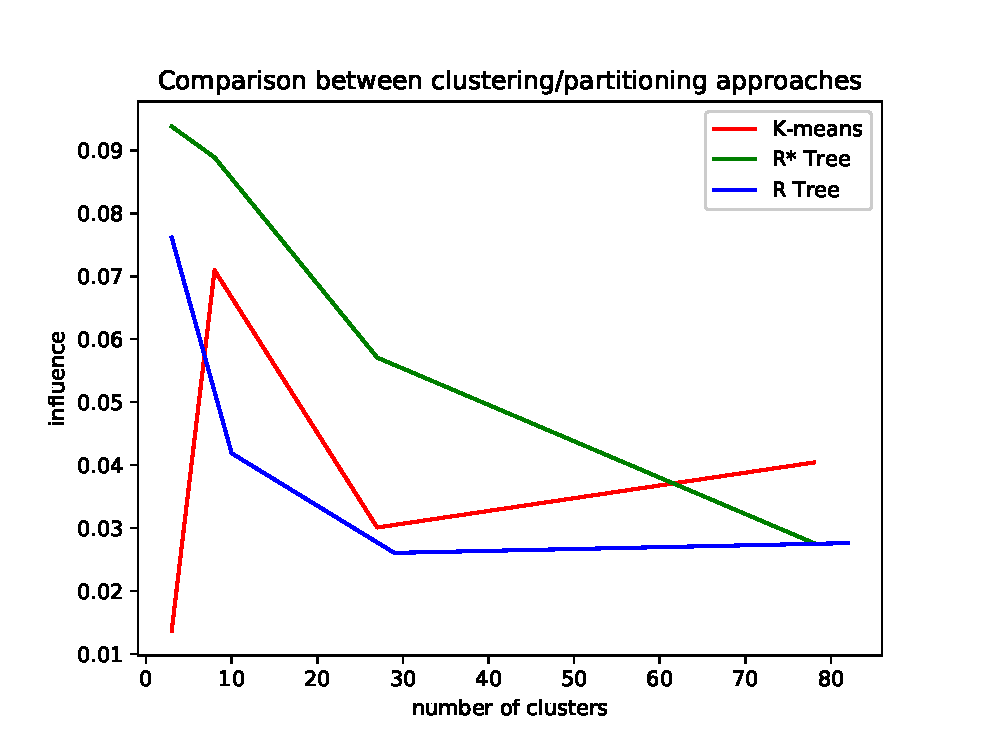
\includegraphics[width=\columnwidth]{clustering_comparison}
\caption{Comparison of Influence against number of clusters for K-Means, R-Tree and R*-Tree}
\label{fig:clustering_comparison}
\end{figure}

K-Means clustering gives a much better result than greedy hierarchical clustering for our problem. However, we also used other spatial partitioning approaches like R-Tree and R*-Tree for comparison. R*-Tree appears to be the partitioning algorithm which gives us the best results according to our experiments. Fig.~\ref{fig:clustering_comparison} shows the comparison between K-Means, R-Tree, and R*-Tree.

% Talk about generating statistics to save time
Once we have our hierarchy set up, we still have to use it to find an explanation. If we had $n$ nodes, the number of clusters we have for our hierarchy is $n \log n$.  This increases the number of combinations of explanations significantly. However, we can use some optimizations to save us some time complexity. Our approach uses memoization of explanations for each spatial node to calculate the value of the degree of explanation. We first calculate the statistics for each node individually and then subtract it from the statistics for the attribute we are observing. For example, let us consider a cluster, $c$, containing two spatial nodes $a$ and $b$. We are interested in the average tip percentage for taxi trips. The degree of candidate explanation by intervention would be the average tip percentage when we remove $a$ and $b$ from our dataset. Our system would memoize the values for the sum and count of tip percentage for $a$, $b$ as $sum_a$, $count_a$, $sum_b$ and $count_b$. It will also calculate the sum and count of tip percentage for the entire dataset. When we need our system to find the degree of explanation for cluster $c$. The formula for average is simply $\frac{sum}{count}$. Since our system calculated all the stats in one query, it does not need to perform additional queries to find the degree. It can simply use $\frac{sum-sum_a-sum_b}{count-count_a-count_b}$ to calculate the average for intervention.

\section{Interface}
We created an interface for the system that we have proposed. This interface is web-based. It consists of a backend server and a front end for visualizations. The Backend is responsible for querying the Apache Spark daemon with relevant queries. The front end allows the user to define observations and visualize explanations. The front end interface makes use of Mapbox to display the map, Deck.gl to create a visualization overlay on the map. The overlay can be points or polygons. In order to handle state changes in the front end, we used React.js front-end library. We also show histograms related to the data. For displaying these histograms, Baidu eCharts library was used. Since the front end was programmed in ES6, webpack was used for transpilation.

In order for the users to easily form observations, our frontend provides them with a series of histograms. Each bar on a histogram represents an aggregate query. Instead of manually writing queries, the user can easily use the bars in the histograms to be used as variables. These variables can then be used in an arithmetic expression representing the user's observations. The user can also define custom variables in the form of aggregate SQL queries manually using the interface.

The back end of the system is an Apache Spark application which calls the Spark daemon for requests of aggravation, intervention, and hierarchical intervention. I must be noted however that there are some operations that the backend performs which are not executed as Spark tasks, such as the creation of an R-Tree.

To allow the front end to communicate with the backend, there is a middleware application. The job of the middleware is to take the input from the front end and execute our backend application with the appropriate function and input parameters. Our middleware is designed using Node Js. It takes aggregate queries, selectivity range and the number of explanations as input and sends it to the backend application. The results are then sent to the frontend.

Fig.~\ref{fig:interface} shows the front end of the web interface that we have designed for helping users find spatial explanations for their observations.

\begin{figure}[h]
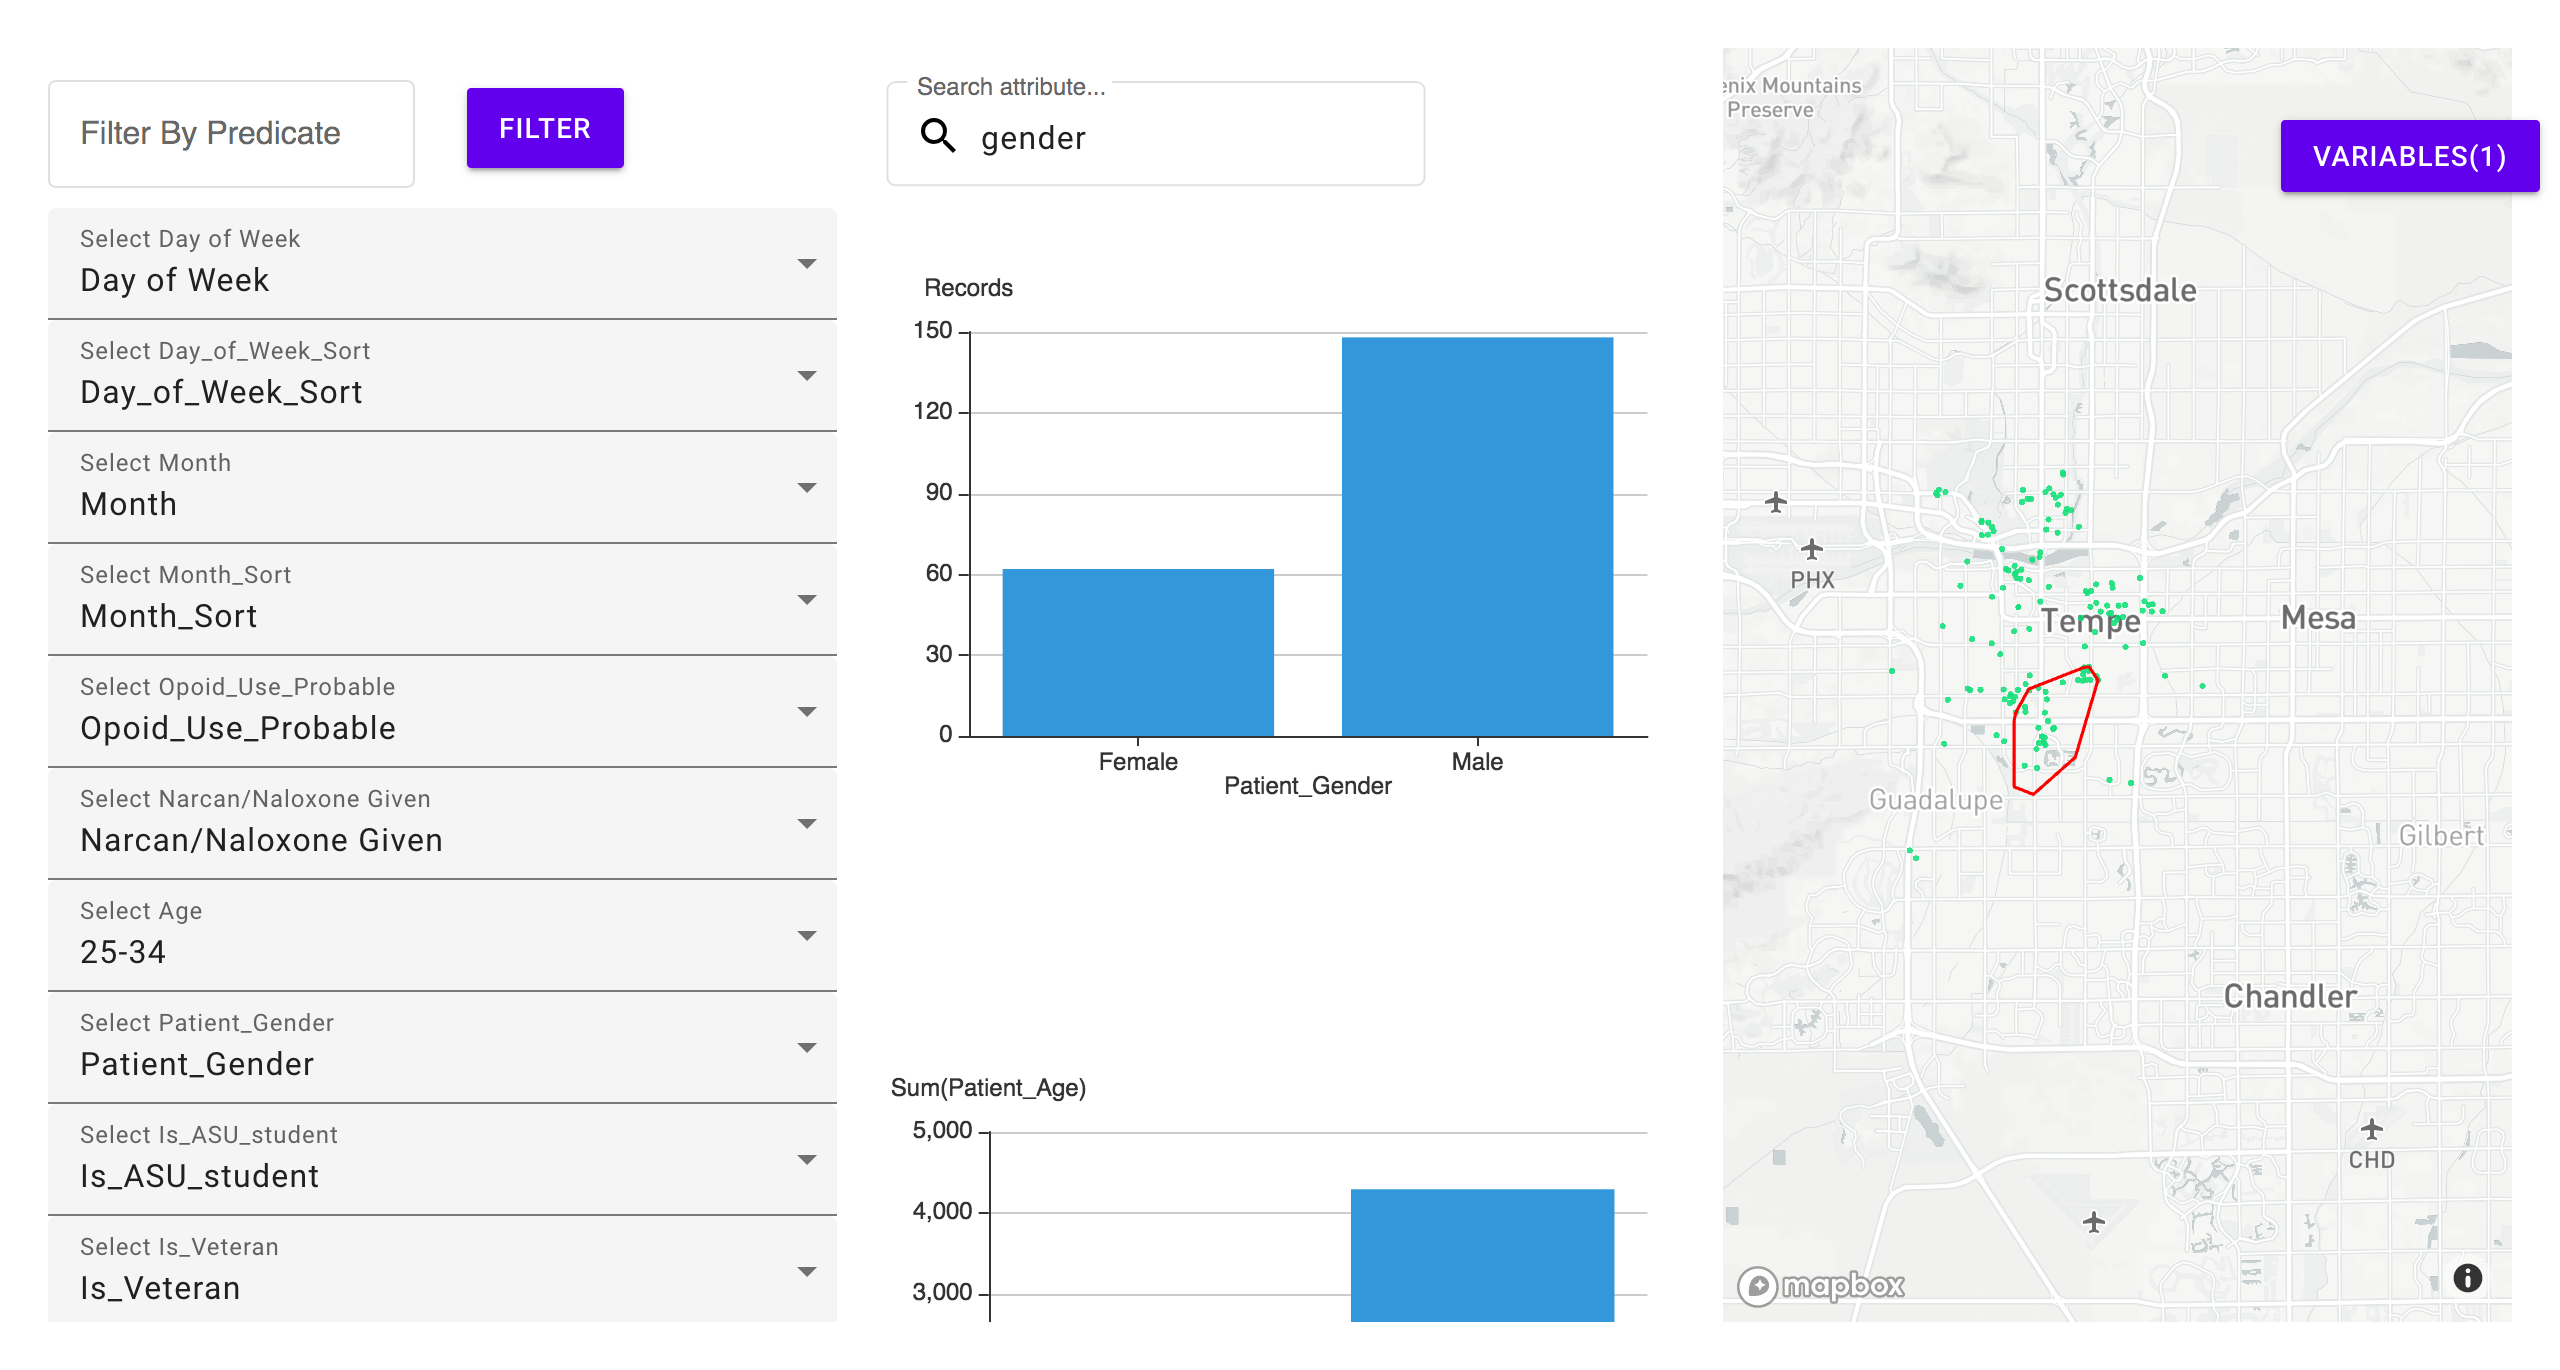
\includegraphics[width=\columnwidth]{interface.png}
\caption{The web interface for our explanation framework}
\label{fig:interface}
\end{figure}
